\newcommand{\bg}[1]{\ensuremath{\boldsymbol{#1}}} 

%-------------------------------------------------
\section{The Schincariol Problem}

%
\DeclareFontFamily{U}{euc}{}
\DeclareFontShape{U}{euc}{m}{n}{<-6>eurm5<6-8>eurm7<8->eurm10}{}%
\DeclareSymbolFont{AMSc}{U}{euc}{m}{n}
\DeclareMathSymbol{\usigma}{\mathord}{AMSc}{27}

\numberwithin{figure}{section}
\numberwithin{equation}{section}
\numberwithin{table}{section}

% Use a new style for remarks
%\theoremstyle{remark}
\newtheorem{rmk}{\textbf {Remark}}
\newtheorem{lemma}{Lemma}
\newtheorem{prop}{Proposition}
\newtheorem{proof}{Proof}
\numberwithin{lemma}{section}
\newtheorem{axiom}{Axiom}
\numberwithin{axiom}{section}

\providecommand{\sembrack}[1]{[\![#1]\!]}
\providecommand{\pD}[2]{\dfrac{\partial #1}{\partial #2}}
\providecommand{\oD}[2]{\dfrac{\mathrm d #1}{\mathrm d  #2}}
\providecommand{\abs}[1]{\lvert #1 \rvert}
%%\providecommand{\abs}[1]{\left\lvert #1 \right\rvert}
\providecommand{\norm}[1]{\left\lVert #1 \right\rVert}
\newcommand{\od}{\mathrm d}

%%%
\newcommand{\js}{\mathscr S}
%%%
%%material index
\newcommand{\pl}{\scriptscriptstyle \mathrm p}
\newcommand{\el}{\scriptscriptstyle \mathrm e}

%%Geometry
\newcommand{\Point}{ \bm x}


%%Displacement field
\providecommand{\Stress}{ \bm \sigma}
\newcommand{\inPStress}{ \Stress_{\imath}} %%% in-plane stress
\newcommand{\stress}{ \sigma}
\newcommand{\devStrs}{\bm s}
\providecommand{\StrainT}{ \bm \epsilon}
\newcommand{\strain}{ \epsilon}
\providecommand{\Disp}{\mathbf u}
\newcommand{\disp}{u}
\newcommand{\vel}{\bf v}
\newcommand{\per}{\mathbf k}
\newcommand{\grv}{\mathbf g}
%%Plasticity
\newcommand{\yld}{ f}
\newcommand{\ppo}{ g}
\newcommand{\pHard}{\mathcal H}
\newcommand{\CT}{\mathbb C}
\newcommand{\DT}{\mathbb D}
\newcommand{\EM}{{\bm C}^{\el}}
\newcommand{\PM}{{\bm C}^{\pl}}
\newcommand{\EPM}{{\bm C}^{\el\pl}}
\newcommand{\mEM}{{\bm D}^{\el}}
\newcommand{\mPM}{{\bm D}^{\pl}}
\newcommand{\mEPM}{{\bm D}^{\el\pl}}
\newcommand{\rdl}{\dot \lambda}
\newcommand{\dl}{\lambda}
\newcommand{\dens}{\rho}
\newcommand{\mnote}{\scriptscriptstyle M}

%%Flow
\newcommand{\densc}{\dens^{\gamma}}
\newcommand{\presc}{p^{\gamma}}
\newcommand{\pres}{p}
\newcommand{\sat}{S}
\newcommand{\Satc}{S^{\gamma}}
\newcommand{\RelKa}{k_{rel}}
\newcommand{\RelK}{k^{\gamma}_{rel}}
\newcommand{\poro}{n}
%%\newcommand{\Fluxf}{\mathbf{v}_{\scriptscriptstyle f}}
\newcommand{\Fluxf}{\mathbf{q}_{\scriptscriptstyle w}}
\newcommand{\Fluxv}{\mathbf{q}_{\scriptscriptstyle v}}
\providecommand{\perm}{ \mathbf k}
\newcommand{\asup}[2]{#1^#2}
\newcommand{\asub}[2]{#1_#2}
\newcommand{\supsub}[3]{{#1}^{#2}_{#3}}
\newcommand{\FlxDf}{\mathbf{J}}
\newcommand{\Sat}{S}

\newcommand{\pn}{\mathbf p}
\newcommand{\pnote}{\scriptscriptstyle f}
%%Heat
\newcommand{\HC}{C_p}
\newcommand{\Flux}{\mathbf{q}}
\newcommand{\Tn}{\mathbf T}
\newcommand{\Tnote}{\scriptscriptstyle T}

%%%FEM
\newcommand{\test}{w}
\newcommand{\Test}{\bm w}
\newcommand{\TestS}{\mathcal V}
\newcommand{\sh}{N}
\newcommand{\Sh}{{\bm N}}
\newcommand{\Mass}{{\mathbf M}}
\newcommand{\Lap}{{\mathbf K}}
\newcommand{\rhs}{{\mathbf f}}

%%Math
\newcommand{\IntD}[1]{{\int}_{\Omega}#1\,\mathrm{d} \Omega}
\newcommand{\intD}{{\int}_{\Omega}}
\newcommand{\intB}{{\int}_{\Gamma}}
\newcommand{\dDom}{\,\mathrm{d} \Omega}
\newcommand{\dBdry}{\,\mathrm{d} \Gamma}
\newcommand{\nrl}{\mathbf n}
\newcommand{\tgl}{\mathbf t}
\newcommand{\I}{\mathbf I}
\providecommand{\domE}[1]{#1^{\alpha}_i}
\def \yieldf {f}
\def \plsp {g}
\def \sivi {\sigma_{v}}
\def \sivii {\mathrm {II}}
\def \siviii {\mathrm{III}}
\def \PlasticParameter {\lambda_p}
\def \devS {\mathbf{s}}
\def \pm {{p_s}}

%%%%%%%%%%%
\def\Kronecker {\boldsymbol{\delta}}
\def\Flux {\mathbf{q}}
\def\FluxFluid {\mathbf{w}}
\def\ElasticityTensor {\boldsymbol{C}}

%bold symbols
\newcommand{\bepsilon}{\boldsymbol{\varepsilon}}
\newcommand{\btau}{\boldsymbol{\tau}}
\newcommand{\bsigma}{\boldsymbol{\sigma}}
\newcommand{\bzero}{\mathbf{0}}
\newcommand{\bv}{\mathbf{v}}
\newcommand{\bw}{\mathbf{w}}
\newcommand{\bx}{\mathbf{x}}
\newcommand{\bz}{\mathbf{z}}
\newcommand{\bt}{\mathbf{t}}
\newcommand{\bu}{\mathbf{u}}
\newcommand{\bq}{\mathbf{q}}
\newcommand{\bn}{\mathbf{n}}
\newcommand{\bg}{\mathbf{g}}
\newcommand{\bk}{\mathbf{k}}
\newcommand{\BX}{\mathbf{B}(X)}
\newcommand{\bK}{\mathbf{K}}
\newcommand{\bN}{\mathbf{N}}
\newcommand{\bC}{\mathbf{C}}
\newcommand{\bI}{\mathbf{I}}
\newcommand{\bff}{\mathbf{f}}
\newcommand{\bp}{\mathbf{p}}
\newcommand{\A}{\mathcal{A}}
\newcommand{\cJ}{\mathcal{J}}
\providecommand{\Div}{\nabla}

%\begin{document} 
%\begin{center}
%\large{\bf Benchmarking density-driven systems aligned orthogonal to gravity in homogeneous porous media}\\
%by Jude L. Musuuza, Florin A. Radu and Sabine Attinger. \\
%%\end{center}
%\normalsize

\subsection{Definition}
The studies investigated the fingering patterns that result when for example saline water intrudes into a confined coastal aquifer. The configuration used in \cite{schinca1} was used where a solute was allowed to flow into the study domain shown in Fig.\ \ref{fig:domain1} with pressure heads maintained over the vertical boundaries to sustain a mean horizontal flow.

%\begin{figure}[!h]
% \centering 
% 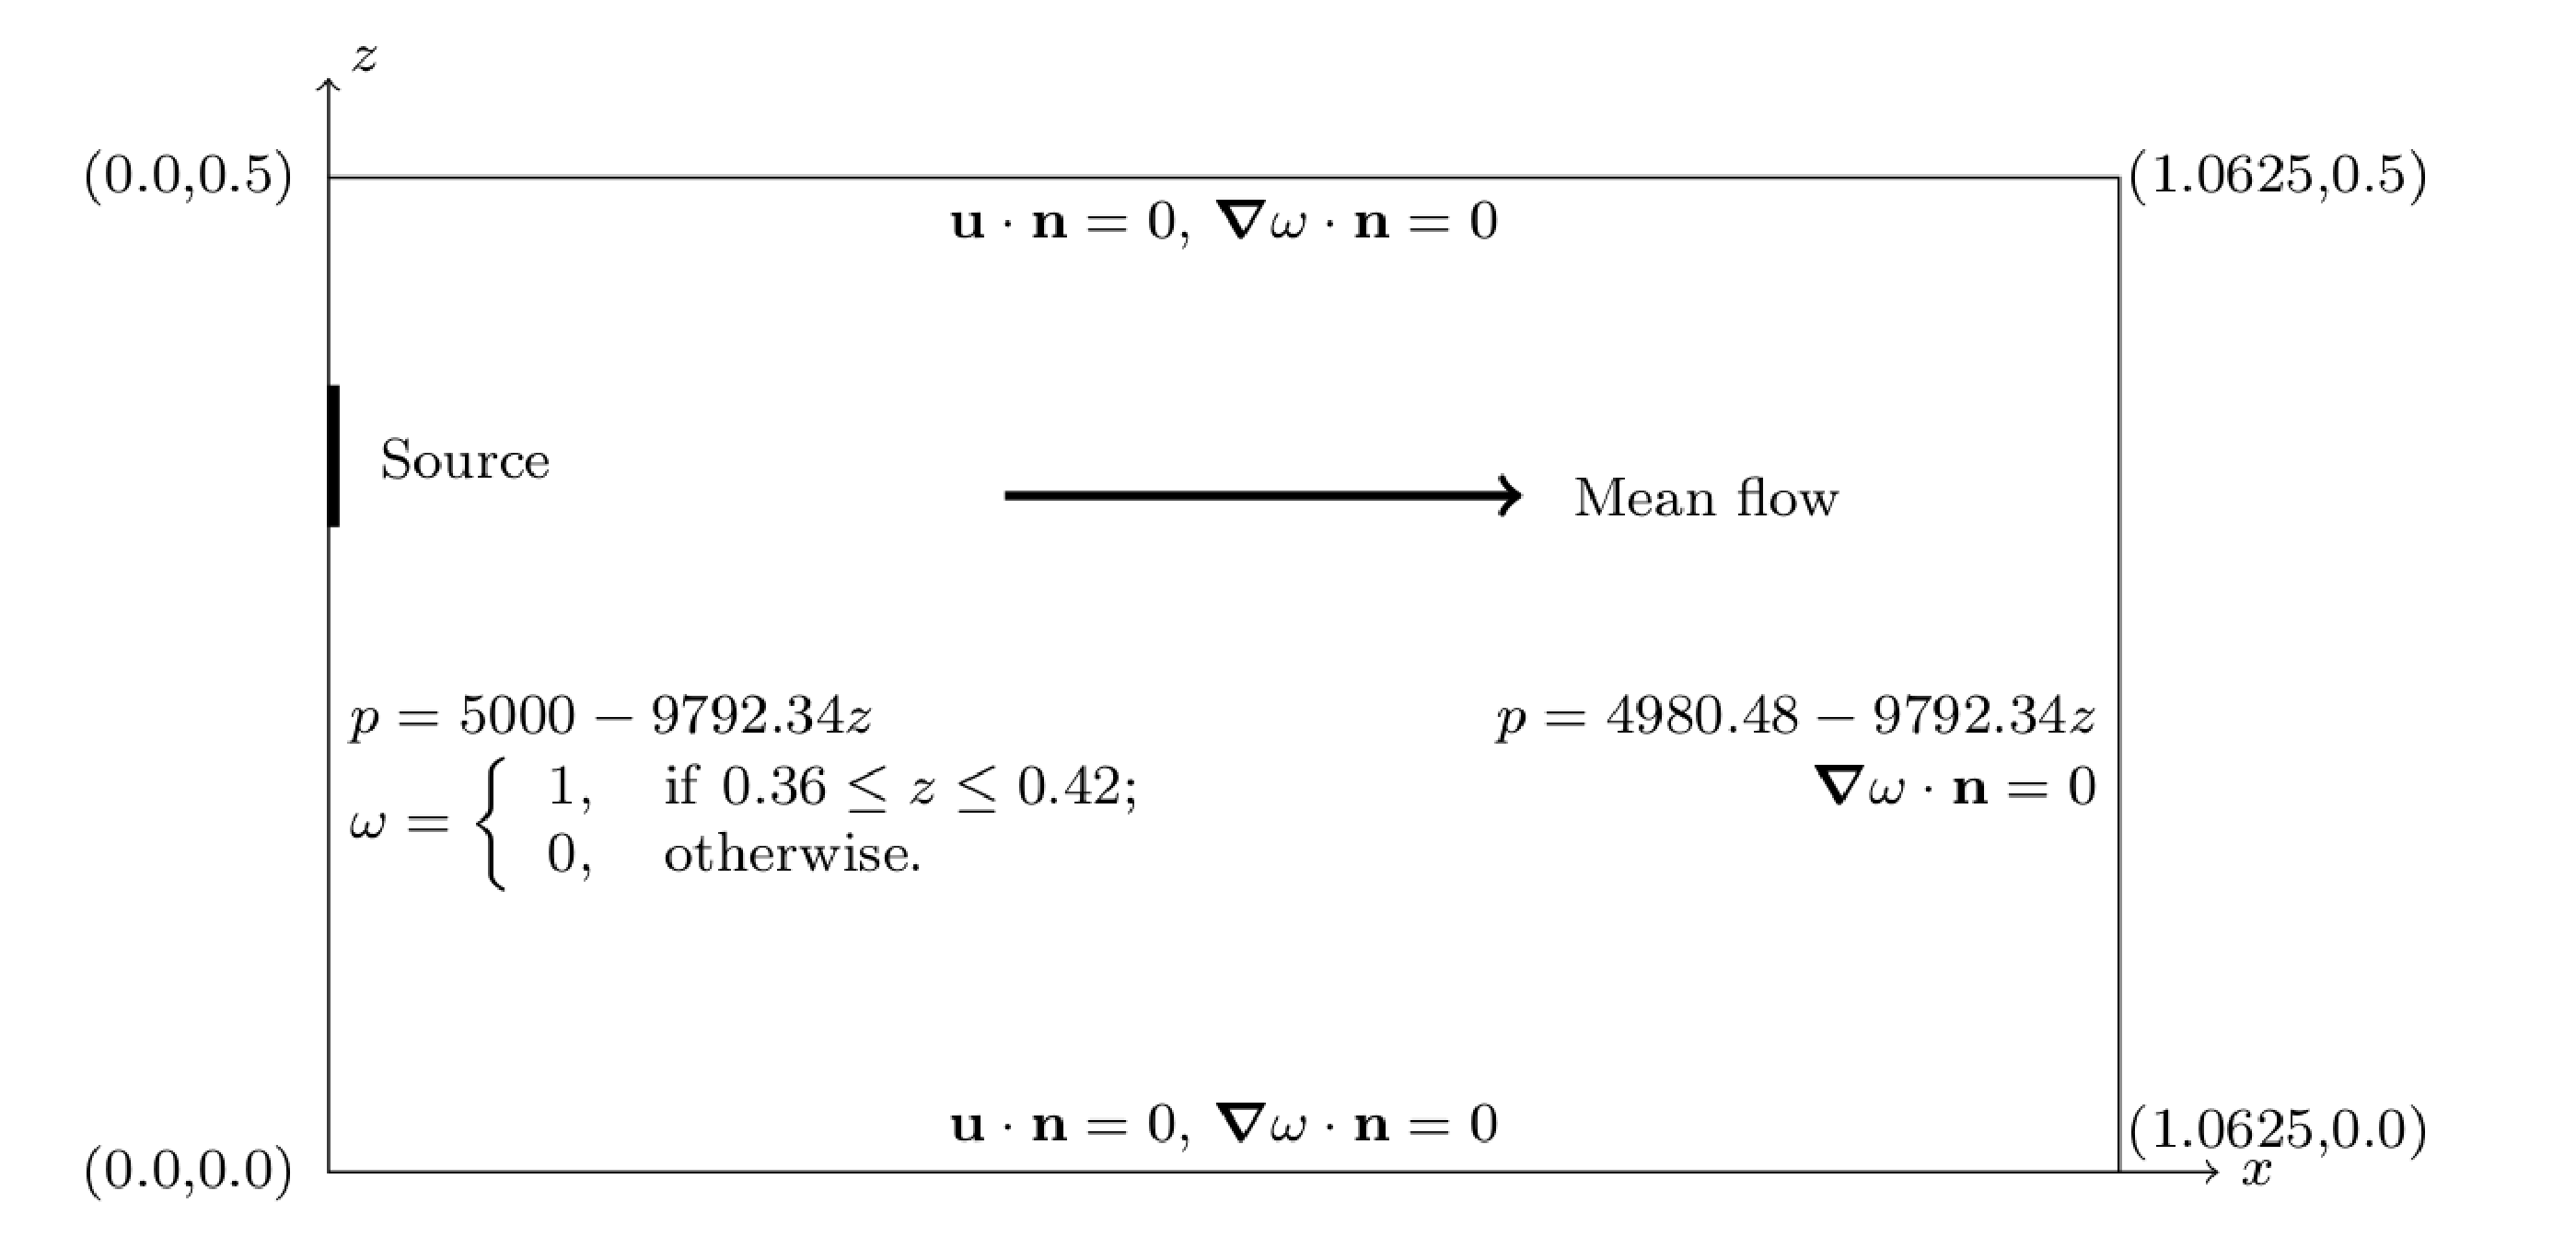
\includegraphics[width=0.85\textwidth] {PART_III/DDF/figures/schincariol_setup}
% \caption{Model set-up}
% \label{fig:domain1}
%\end{figure}

\begin{figure}[!ht]
\begin{center}
\begin{tikzpicture}%[thin]
\draw (0,0) rectangle (9.0,5.0);
{\scriptsize
\draw[fill=black] (0,3.25)rectangle(0.05,3.95);
\draw (0.15,3.59) node[anchor= west]{Source};
\draw(0.0,1.75) node[anchor=west]{$\omega=\left\{\begin{array}{rl}
                                                    1,&{\rm if }\,\,0.36\le z\le 0.42;\\
                                                    0,&{\rm otherwise.}\\
                                                    \end{array}\right.$};
\draw(0.0,2.27) node[anchor=west]{$p=5000-9792.34z$};
\draw(9.0,1.95) node[anchor=east]{${\bg{\nabla}\omega} \cdot {\bf n} = 0$};
\draw(9.0,2.27) node[anchor=east]{$p=4980.48-9792.34z$};
\draw(4.5,0.0) node[anchor=south]{${\bf u} \cdot {\bf n} = 0,\,\bg{\nabla}\omega\cdot{\bf n} = 0$};
\draw(4.5,5) node[anchor=north]{${\bf u} \cdot {\bf n} = 0,\,\bg{\nabla}\omega\cdot{\bf n} = 0$};
\draw(-0.7,0) node{\scriptsize(0.0,0.0)};
\draw(-0.7,5) node{\scriptsize(0.0,0.5)};
\draw(9.8,0.2) node{\scriptsize(1.0625,0.0)};
\draw(9.8,5) node{\scriptsize(1.0625,0.5)};
\draw [very thick,->](3.4,3.4)--(6,3.40);
\draw (6.15,3.4) node[anchor= west]{Mean flow};
\draw [->](9,0)--(9.5,0);
\draw (9.5,0) node[anchor= west]{$x$};
\draw [->](0,5)--(0,5.5);
\draw (0,5.6) node[anchor= west]{$z$};
}
\end{tikzpicture}
\end{center}
 \addtolength{\abovecaptionskip}{-0.5cm}\caption{\label{fig:domain1} Model set-up}%
\end{figure}

\paragraph*{Domain setup.} Using the simulation parameters in Table \ref{tab:simu}, the grid and time steps were refined until a solution free of numerical artifacts was obtained.
\begin{table}[!h]
{\footnotesize
\begin{center}
\caption{\label{tab:simu}Simulation parameters}
\begin{tabular}{|l|l|l|l|}\hline
{\bf Parameter}                                 &{\bf Notation}     &{\bf Value}            &{\bf Unit} \\\hline\hline
Porosity                    &$\phi$          &$0.38$             &--     \\
Molecular diffusion coefficient of NaCl     &$D_m$          &$1.61\times 10^{-9}$   &$m^2\cdot s^{-1}$  \\
Longitudinal dispersivity           &$\alpha_{\parallel}$     &$1.0\times 10^{-3}$        &$m$        \\
Transverse dispersivity             &$\alpha_{\perp}$      &$2.0\times 10^{-4}$      &$m$        \\
Mean flow velocity             &$v_{0}$      &$2.75\times 10^{-6}$      &$m\cdot s^{-1}$        \\
%Pressure-driven velocity component     &$v_0^p$        &$2.75\times 10^{-6}$       &$m\cdot s^{-1}$    \\
%Gravity-driven velocity                         &${\bf v}^g$            &$5.57\times 10^{-4}$          &$m\cdot s^{-1}$\\
%Norm of velocity                               &$\Nor{v}$              &$5.57\times 10^{-4}$           &$m\cdot s^{-1}$\\
Domain Length in flow direction                 &$L$                    &1.0625                         &$m$\\
Viscosity of pure water at $20^{\circ}C$      &$\mu_0$        &$1.002\times 10^{-3}$      &$Pa\cdot s$        \\
Maximal viscosity of solution (2000mg/l NaCl at $20^{\circ}C)$  &$\mu_{max}$  &$1.006\times 10^{-3}$      &$Pa\cdot s$        \\            
Density of pure water at $20^{\circ}C$        &$\rho_0$       &998.2          &$kg\cdot m^{-3}$   \\
Maximal density of solution (2000mg/l NaCl at $20^{\circ}C)$                  &$\rho_{max}$       &999.7          &$kg\cdot m^{-3}$   \\
%Maximal solute mass fraction           &$\omega_{max}$     &1.0            &--     \\
%Maximum relative viscosity coefficient     &$\beta$        &$3.99\times 10^{-3}$       &--     \\
%Maximum relative density coefficient       &$\alpha$       &$1.507\times 10^{-3}$      &--     \\
Tortuosity                 &$\varsigma$      &0.35               &--     \\
Gravity vector                  &{\bf g}        &-9.81              &$m\cdot s^{-2}$    \\
%Maximal density of NaCl at $20^0C^\star$                  &$\rho_{max}$       &998.5          &$kg\cdot m^{-3}$   \\
%Longitudinal dispersivity$^\star$           &$\Lon{\alpha}$     &$1.5\times 10^{-3}$        &$m$        \\
%Transverse dispersivity$^\star$          &$\Pp{\alpha}$      &$1.0\times 10^{-4}$      &$m$        \\
%Domain Length in flow direction$^\star$                &$L$                    &1.1                         &$m$\\
%Horizontal concentration gradient      &$G_1$              &-0.00188           &$m^{-1}$       \\
%Vertical concentration gradient                &$G_2$              &1.0            &--     \\
%Vertical correlation length                     &$\lambda_v$              &0.0075                  &$m$\\
%Horizontal correlation length                   &$\lambda_h$              &0.0075                  &$m$\\
Mean permeability                    &$k_{0}$        &$5.7\times 10^{-11}$  &$m^2$      \\\hline
%Heterogeneity variance                                        &$\sigma^2$             &0.60                                   &-\\\hline
\end{tabular}
\end{center}
}
\end{table}

\subsection{Results}
Their results at the approximate P\`{e}clet and Courant numbers were nearly exactly reproduced in \cite{musu} as shown in Fig.\ \ref{fig:stand}. The P\`{e}clet and Courant numbers reported in the figure were obtained with mesh sizes of 0.3 with 4 refinements and a time step of 1hr; 0.3 with 5 refinements and a time step of 45min; and 0.2 with 5 refinements and a time step of 57min. The reproducibility of the results makes the problem defined by \cite{schinca1} a suitable reference from which further investigations can be founded. 
\begin{figure}[!h]\footnotesize
  \begin{center}
    \subfigure[Pe=16.5, Cr=0.22]{\label{fig:stand1}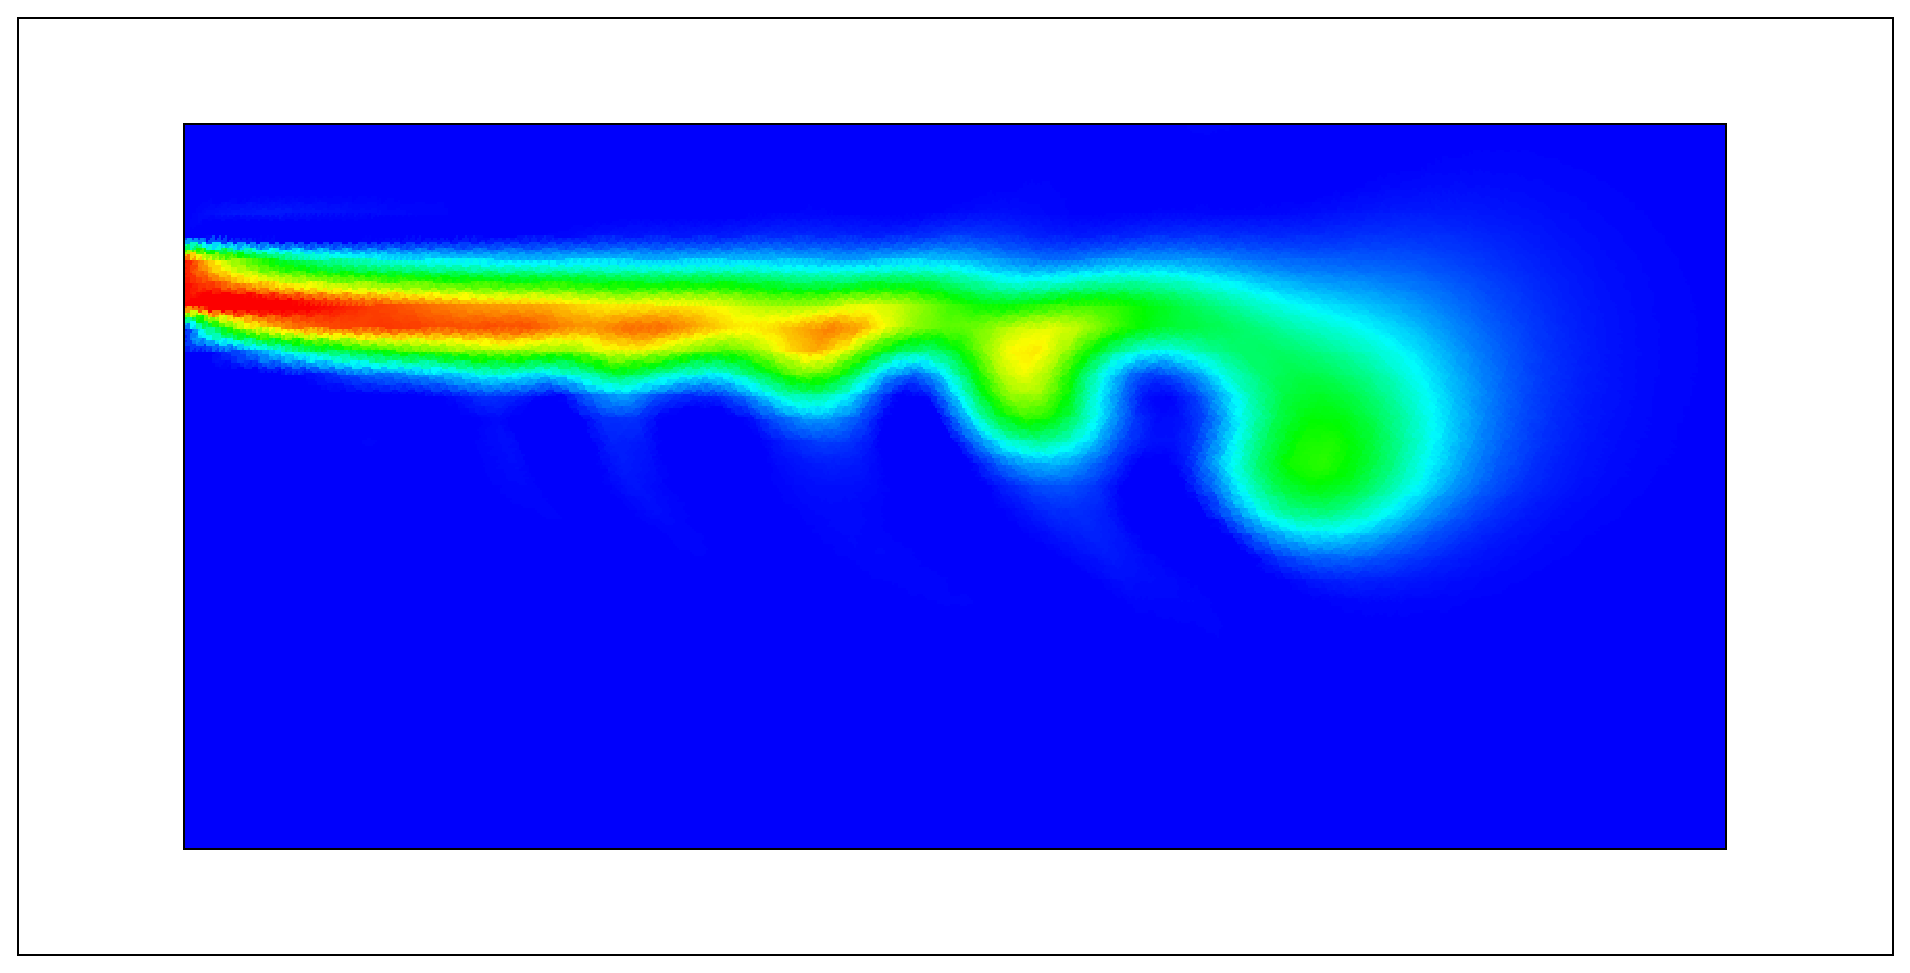
\includegraphics[scale=0.14,clip,viewport=89 52 809 399]{PART_III/DDF/figures/schincariol_schi1}}\hspace{0.2cm}
    \subfigure[Pe=8.40, Cr=0.40]{\label{fig:stand2}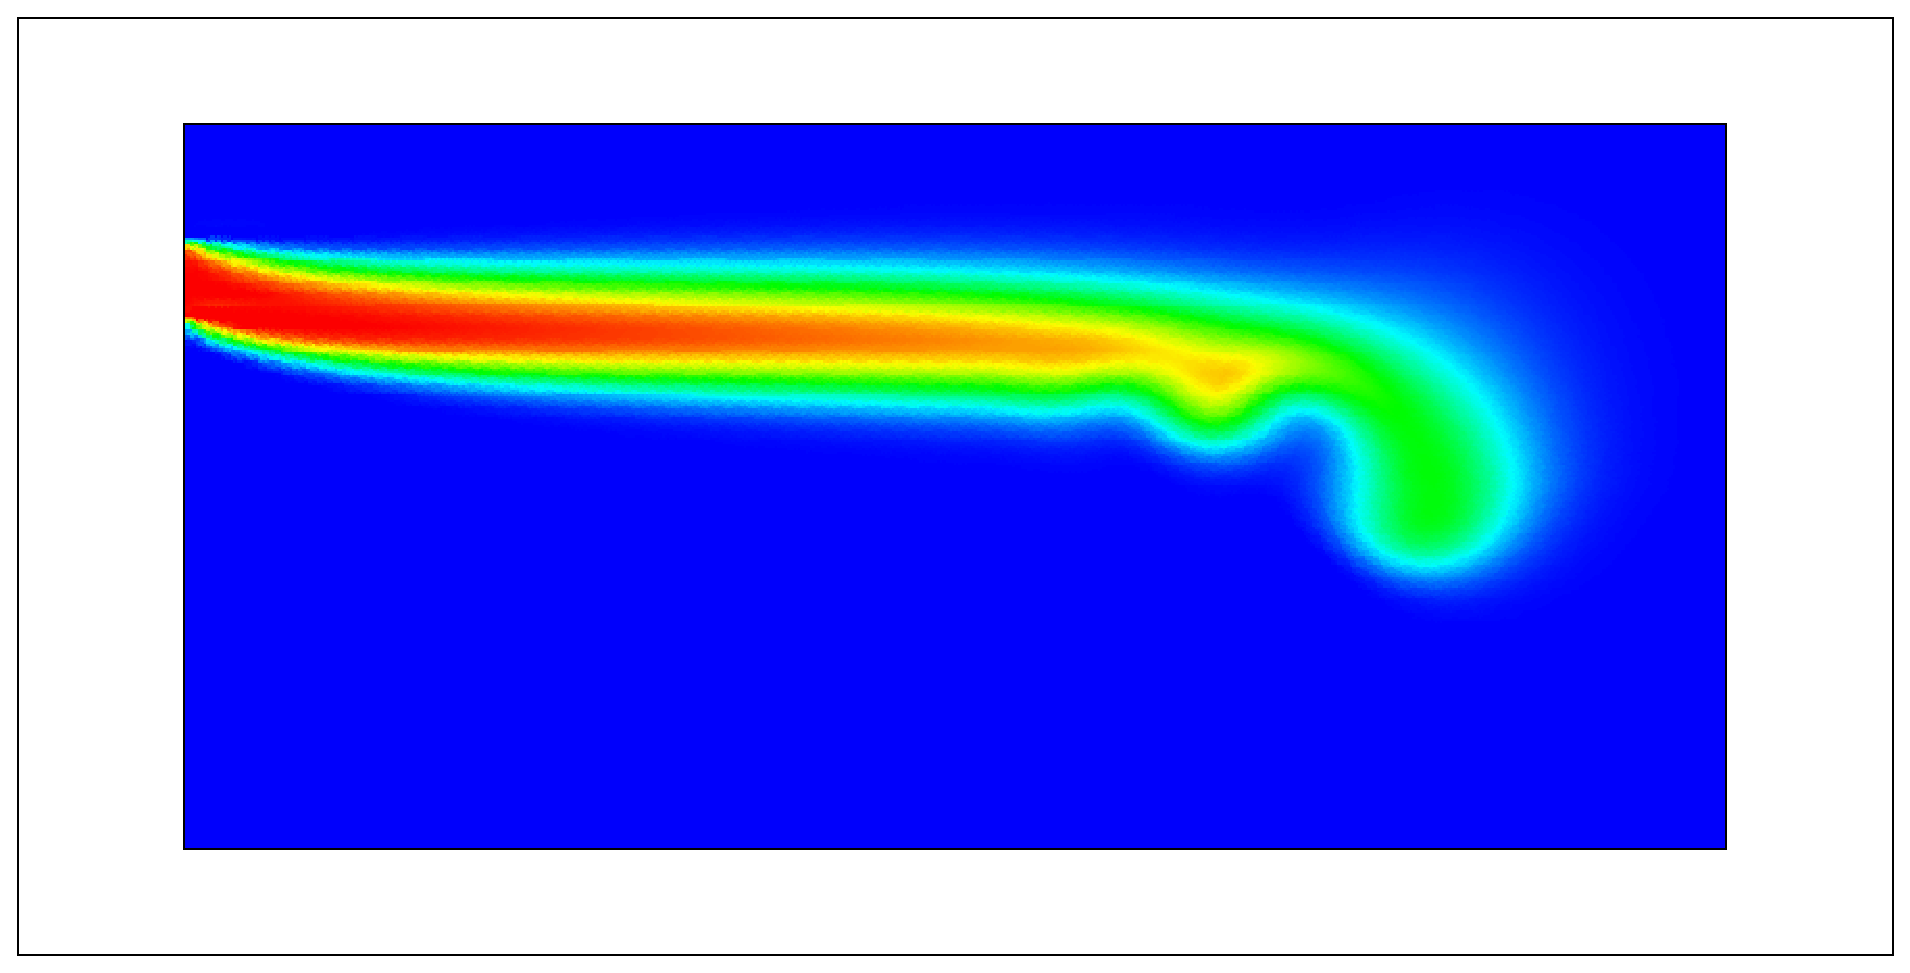
\includegraphics[scale=0.14,clip,viewport=89 52 809 399]{PART_III/DDF/figures/schincariol_schi2}}\hspace{0.2cm}
    %\subfloat[Pe=5.50, Cr=0.75]{\label{fig:stand3}\includegraphics[scale=0.155,clip,viewport=89 52 809 399]{schi3}}
    \subfigure[Pe=2.32, Cr=1.10]{\label{fig:stand4}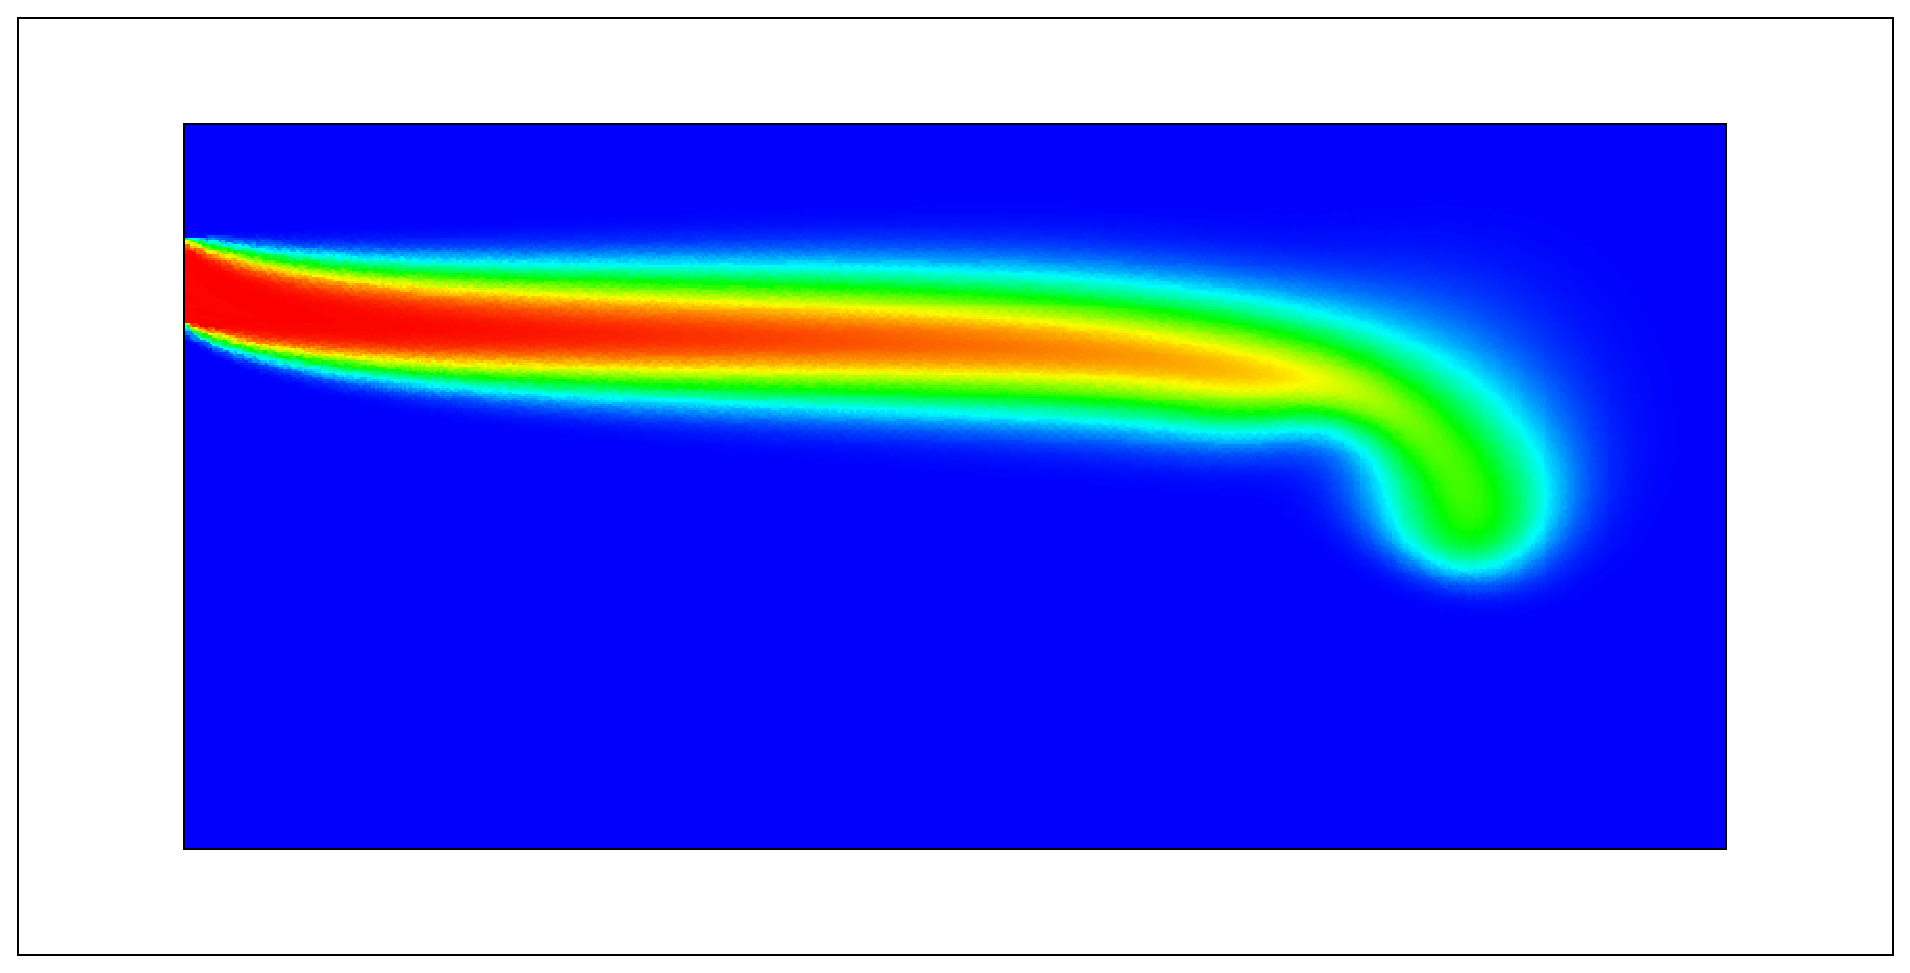
\includegraphics[scale=0.14,clip,viewport=89 52 809 399]{PART_III/DDF/figures/schincariol_schi4}}
  \end{center}
  \addtolength{\abovecaptionskip}{-0.45cm}\caption{\label{fig:stand} A reproduction of Schincariol results with full equations}
 \end{figure}

Due to the rotation of the velocity field caused by density variations in the boundary layer,  some salt accumulates and is trapped in the tip of the of the plume. Therefore, the ever-present lobe at the tip does not count as a finger and Fig.\ \ref {fig:stand4} is considered to be free from instabilities. That numerically stable configuration was further used by \cite{schinca1} to study the effect of periodically varying the width of the inflow region and by \cite{schinca2} to study the effect of medium heterogeneity on fingering patterns. It was also used in \cite{musu} to investigate the effects of physical variables like density, viscosity and flow velocity on the evolution of fingers. 

Sample results from numerical studies in \cite{musu} without the Oberbeck-Boussinesq approximation are shown in Fig.\ \ref{fig:ob}.
%\begin{figure}[!h]\footnotesize
%  \begin{center}
%    \subfloat[$\rho=999.7\,kg\cdot m^{-3}$]{\label{fig:ob1}\includegraphics[scale=0.155,clip,viewport=81 53 820 401]{d9997}}\hspace{0.2cm}
%    \subfloat[$\rho=1000.4\,kg\cdot m^{-3}$]{\label{fig:ob4}\includegraphics[scale=0.155,clip,viewport=81 53 820 401]{d10004}}\hspace{0.2cm}
%    \subfloat[$\rho=1002.0\, kg\cdot m^{-3}$]{\label{fig:we4}\includegraphics[scale=0.155,clip,viewport=81 53 820 401]{w4}}
%  \end{center}
%  \addtolength{\abovecaptionskip}{-0.45cm}\caption{\label{fig:ob} Fingering patterns at various densities}
% \end{figure}


\begin{figure}[!h]\footnotesize
  \begin{center}
    \subfigure[$\rho=999.7\,kg\cdot m^{-3}$]{\label{fig:ob1}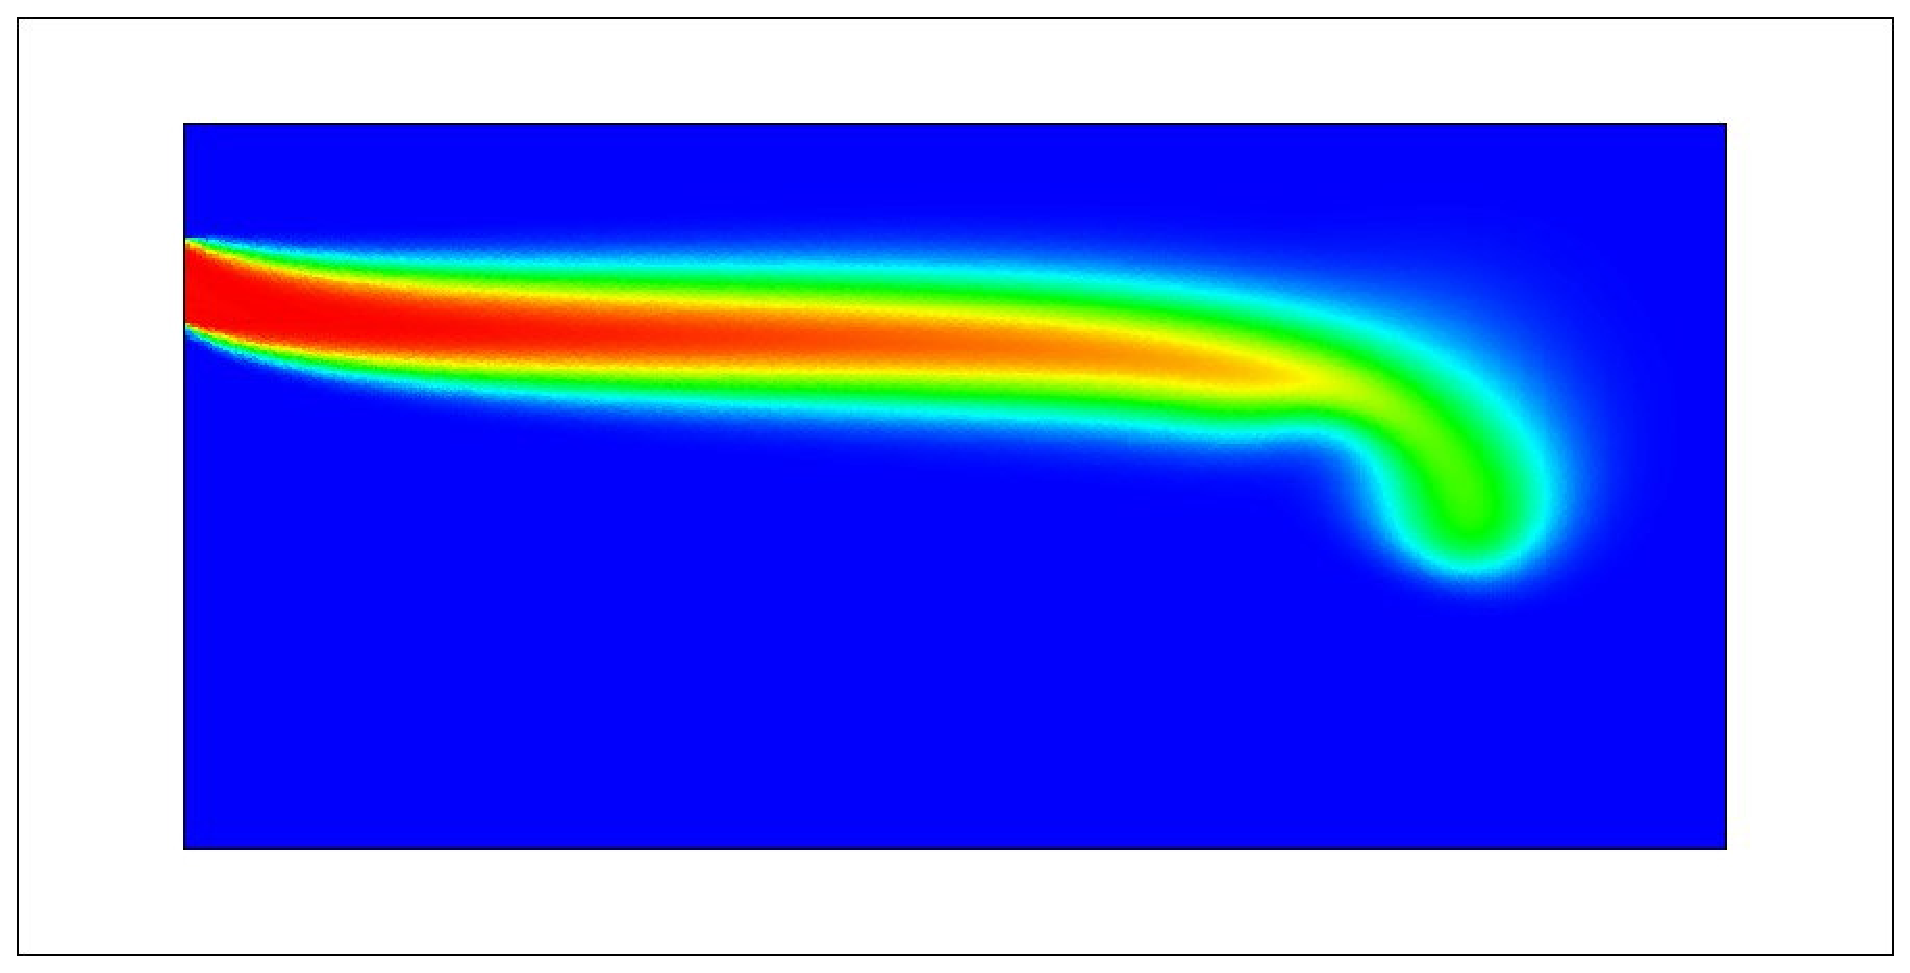
\includegraphics[scale=0.14,clip,viewport=81 53 820 401]{PART_III/DDF/figures/schincariol_d9997}}\hspace{0.2cm}
    \subfigure[$\rho=1000.4\,kg\cdot m^{-3}$]{\label{fig:ob4}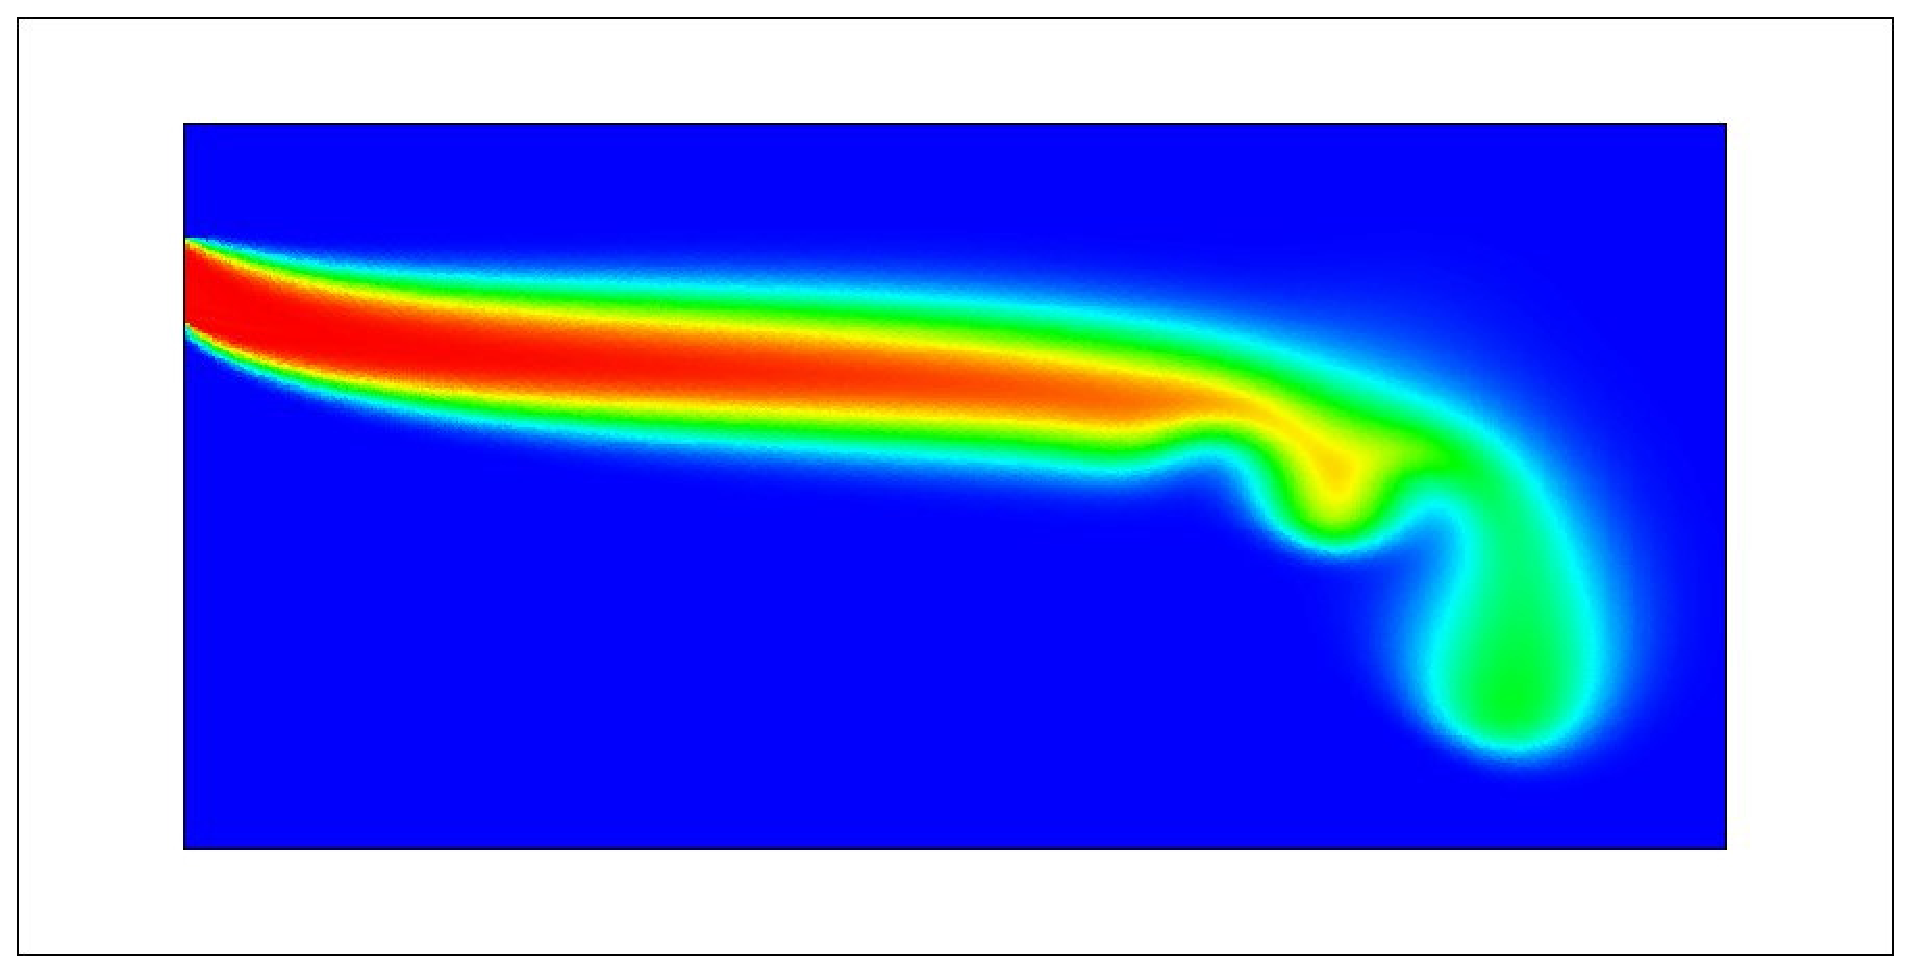
\includegraphics[scale=0.14,clip,viewport=81 53 820 401]{PART_III/DDF/figures/schincariol_d10004}}\hspace{0.2cm}
    \subfigure[$\rho=1002.0\, kg\cdot m^{-3}$]{\label{fig:we4}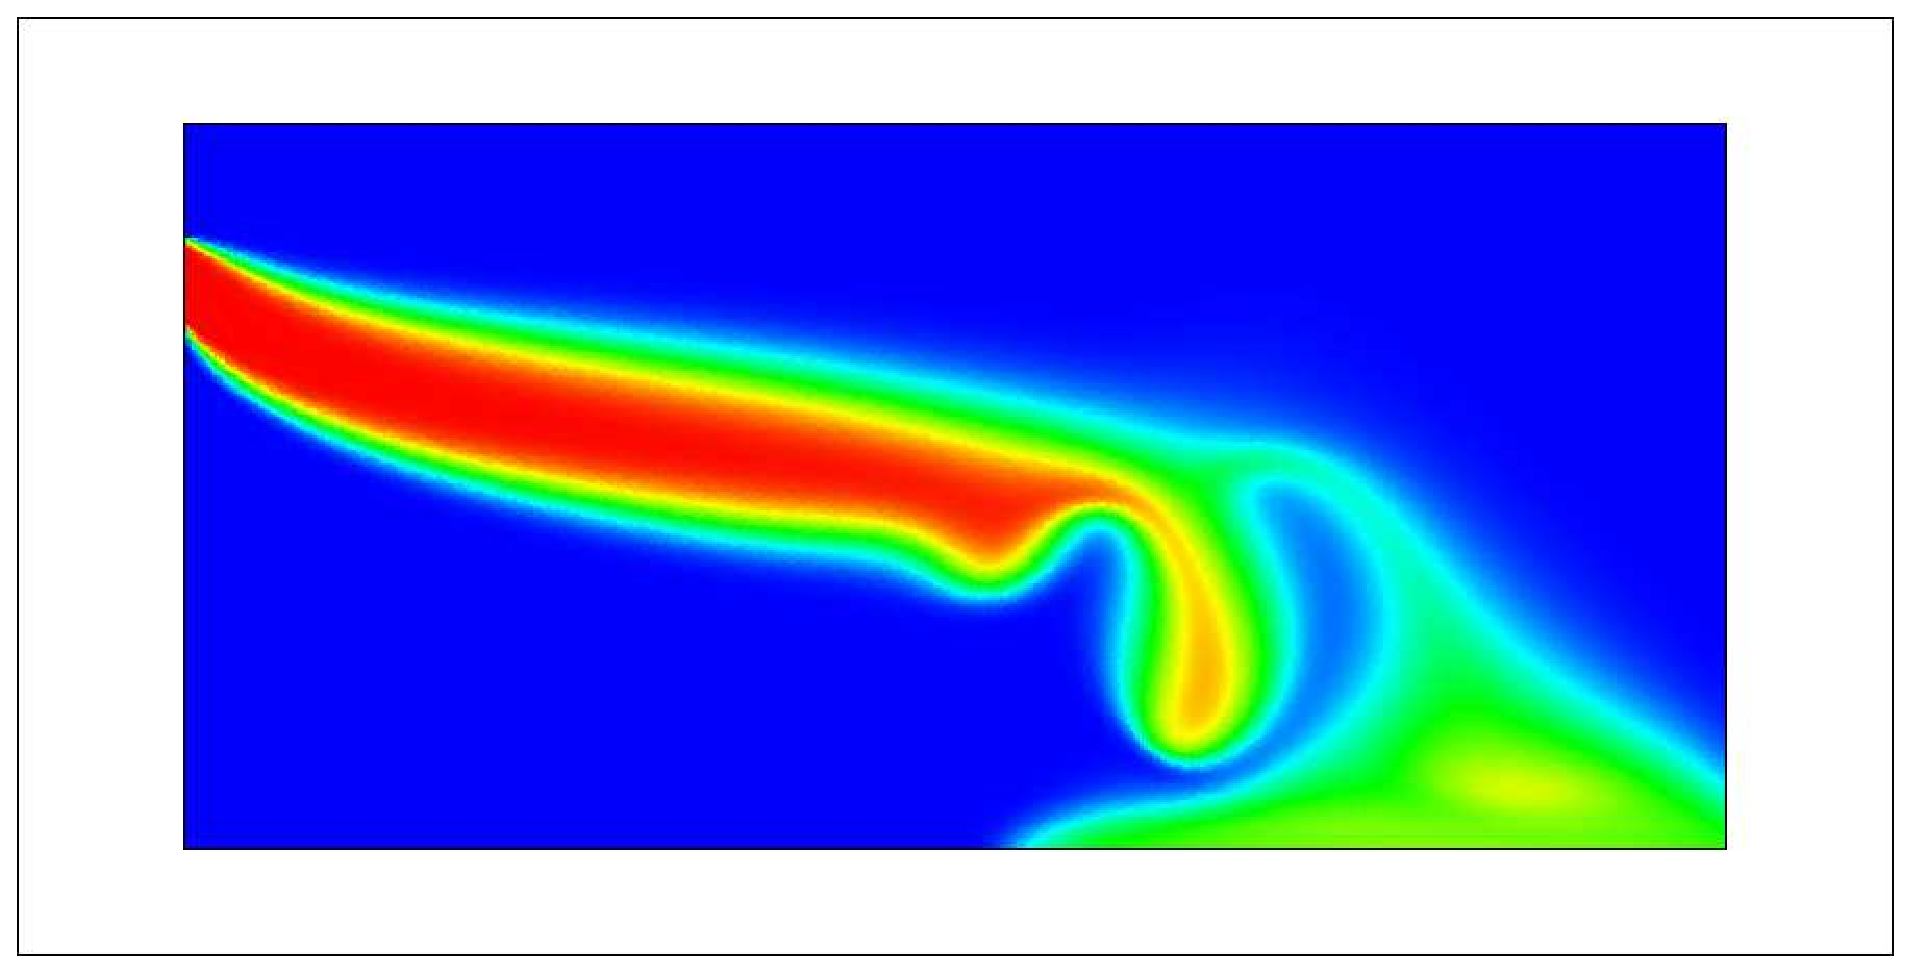
\includegraphics[scale=0.14,clip,viewport=81 53 820 401]{PART_III/DDF/figures/schincariol_w4}}
  \end{center}
  \addtolength{\abovecaptionskip}{-0.45cm}\caption{\label{fig:ob} Fingering patterns at various densities}
 \end{figure}



%\footnotesize
%\bibliography{authors}     %Path for bibliography
%\end{document}